\chapter{if conversion \Author{C. Bruel}}
\numberofpages{10}
\graphicspath{{img/}{if_conversion/img/}{part4/if_conversion/img/}}
	
\newcommand\cond{~?~}

TODO: compare speculation and predication dependence height
TODO: example with branch probabilities and beneficibility
TODO: running example on complex region
TODO: ?

\section{Overview/Motivations}

In \ref{ferriere:sec:psi-ssa} $\psi$-SSA was described as a way to express a predicated form of SSA extension. Such representation is usually built from already predicated code, non SSA, originating from inlined assembly, peepholes, intrinsics functions or local transformations of control flow idioms.

If-conversion is a global process to remove conditional branches by transforming a control flow region into a single equivalent basic block, replacing conditional control flow execution by a sequence of conditional instructions. 

Removing branches improves performance in several ways: by removing the mis-prediction penalty, the instruction fetch throughput is increased and the instruction cache miss penalty reduced. Enlarging the size of the basic blocks allows the static scheduler to schedule earlier long latencies operations and to improve the ILP by merging multiple flows of execution, with an optimized allocation of the different data paths. 

Several algorithmic or design choices impact the effectiveness of if-conversion. As an optimization, the region to if-convert, e.g hyperblock, must be just large enough to have the largest scope of scheduling framework, but in the same time it must not over-commit the machine resources (registers, CPUs). On the contrary, although if-conversion removes branches, I also add some overhead (new instructions to merge predicates, register pressure for speculative conditional, bigger dependence height because of the presence of new data dependencies on the predicates). The newly formed basic block doesn't have a higher schedule estimation than the one that would have been taken if the code was not if-converted.

For this reason, existing approaches of if-conversion are either local using peepholes or intrinsics, or scoping larger but restricted regions such as loops hyperblocks. Such approaches require that the region is isolated from the rest of the control flow, for instance using tail duplication (cause for code bloat), and more important requires a complicated estimation of the future if-converted region. So many factor impact this (predicate computation, register pressure, dependence height) that the objective function needs to be very conservative. Traditionally if-conversion cover the following steps:

\begin{itemize}
\item Isolate the control flow region for which if-conversion is beneficial, using predictive heuristics. Using tail duplication to remove incoming edges. For example using the Hyperblock framework.
\item Compute and assign a predicate to each basic block.
\item Convert the instructions into predicated ones using the predicate computed from the basic block, and merge the basic blocks.
\item Apply some predicate reduction mechanism to simplify predicate equations.
\item Finally emit the newly predicate computations and the predicated code. If the ISA is not fully predicated, an additional pass is needed to conditionalize them using conditional moves only.
\end{itemize}

All those operations make the if-conversion process a complex optimization, forcing designers to be extremely conservative, as the objective functions must contain variables not known at the start of the transformation. (such as the complexity of the predicate equations) since moving multiple control paths together can easily exceed processors resources (leading to excessive register pressure) or move infrequently used expensive instruction (memory loads) into the critical path. 

The SSA framework allows the decision functions to be accurate enough to avoid being too conservative and aggressively if-convert code, we will see in this chapter than an iterative bottom up process, on the SSA form can be more efficient, and more effective than the traditional top down techniques.

\subsection{Architectural requirements}
Conditional operations can be done thanks to different ways (predication, speculation, conditional moves and requires predicate computation and merge operation). The SSA framework described here supports a mix, or all of those ways. We suppose that the target architectures has a way to emit conditional execution of instruction. This is usually achieved in 3 different ways: In this chapter we use following notation for the simple $x = p \cond a + b : 0$ assignment.

\begin{figure}
\begin{minipage}[t]{4cm}
\mbox{fully predicated:} \\
$ p \cond x = a + b $ \\
$ \overline{p} \cond x = 0 $ \\
\end{minipage}
\begin{minipage}[t]{4cm}
\mbox{partially predicated:} \\
$t = a + b $ \\
$p \cond x = t $ \\
$\overline{p} \cond x = 0 $ \\
\end{minipage}
\begin{minipage}[t]{4cm}
\mbox{$select$ instruction:} \\
$t = a + b $ \\
$x = select \; p \cond t : 0 $ \\
\end{minipage}
\end{figure}

\subsection{SSA if-conversion overview}

Locally, we notice then if-conversion require two problems to be solved.
\begin{itemize}
\item A renaming problem to avoid the multiple definitions of a different variables assignment merged into a single path. 
\item Minimize the number of instructions to be predicated. Only instruction that merge need to be conditionalized inside the predicate set that control the merge. Others can be safely speculated without the need of a special predicate reduction pass. 
\end {itemize}

SSA \cite{BriggsSSA} provides an efficient intermediate representation in which all false data dependencies have been removed, thus removing the need for register renaming needed when merging two definitions into one. Each assignment target (def) is assigned a unique register name. Registers are re-materialized at join nodes using $\phi$ operations. A procedure is in minimal SSA form if the number of $\phi$ instructions at join nodes is as small as possible. SSA-form representation gives the properties that a variable is assigned only once, and their merging point is exposed info $\phi$ operations solves those problems. 

Once the operations to be conditionalized have be isolated. The framework still need to answer two other questions: As a global problem the region to if-convert must be defined, using objective functions and branch probabilities to avoid moving to the hot path less frequently used instruction. Since if-conversion also transforms control flow dependencies into data flow dependencies, register pressure can become significantly high. Such decision function must take into account operations created by the process itself, such as predicate merging or new copies. 

Locally, for each basic block considered into the region, a predicate must be computed and assigned to the corresponding instructions. Finally predicated or speculative instructions must be emitted into the IR, and the SSA IR maintained. Note that basically, Since a SSA $\phi$ express the merging point of $n$ definitions from $n$ predecessors, we can safely say the the definition points depends on their nearest condition under which they depend. Intuitively we already know that thanks to SSA the definition point is straightforward to find. Definitions not merging into a $\phi$ don't need to be conditionalized

This algorithm takes as input SSA form and produces either $\psi$-SSA if predicated instructions are available or pure SSA using select instructions to realized join points.

\subsection{SSA representation of conditional instructions}

$\psi$-SSA expose the edge dependency from the basic block into which the definitionition of the $\phi$ argument is defined in the original CFG by a new data dependency. This dependency needs to be matemarialized into a $select$ or $\psi$ operation. Note that the $select$ operation is a real instruction that don't need to be replaced by the out-of-ssa process. If the target architecture doesn't provide such instruction to switch between speculated instruction, it can be emulated using two conditional moves. One advantage to generate $select$ instruction at this stage is that the program stays in full SSA form and make all the data dependencies explicit, and can be feed to all SSA optimizers. 

\begin{figure}
\begin{minipage}[t]{4cm}
\mbox{SSA:} \\
$ if (p) $ \\
$   x_1 = a+b $ \\
$ else $ \\
$   x_2 = 0 $ \\
$ x = \phi (x_1, x_2) $ \\
\end{minipage}
\begin{minipage}[t]{4cm}
\mbox{SSA-speculative form:} \\
$x_1 = a + b $ \\
$x_2 = 0 $ \\
$x = select p ? x_1, x_2$ \\
\end{minipage}
\begin{minipage}[t]{4cm}
\mbox{$\psi$-SSA form:} \\
$x_1 = a + b $ \\
$x_2 = 0 $\\
$x = \psi (p \cond x_1, \overline{p} x_2) $ \\
\end{minipage}
\end{figure}

Note that unlike $\phi$ arguments are executed simultaneously (they don't depend each other), $\psi$ arguments are executed sequentially and ordered from their definition predicate set. This propriety is necessary because if-conversion replaces the ``spacial'' dependency from the CFG by a ``temporal'' dependency from the straight line predicated code.

\subsection{SSA operations on basic blocks}

We first start to describe the local operations, that will be the basis, by iterative transformations for the region construction process. 

\begin{figure}
\begin{minipage}[t]{5cm}
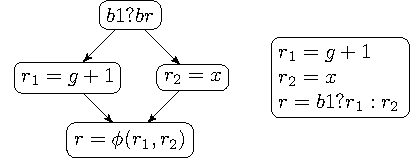
\includegraphics[scale=0.2]{phi_removal.pdf}
\caption{phi removal}
\label{fig:phi_rem}
\end{minipage}
\begin{minipage}[t]{5cm}
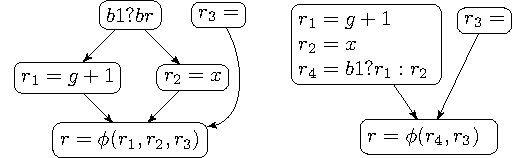
\includegraphics[scale=0.2]{phi_reduction.pdf}
\caption{phi reduction}
\label{fig:phi_red}
\end{minipage}
\begin{minipage}[t]{6cm}
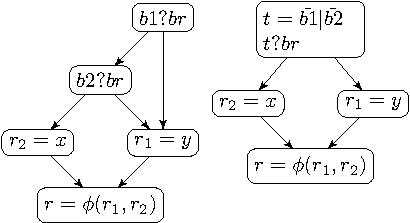
\includegraphics[scale=0.2]{phi_merge.pdf}
\caption{predicate merge}
\end{minipage}
\begin{minipage}[t]{5cm}
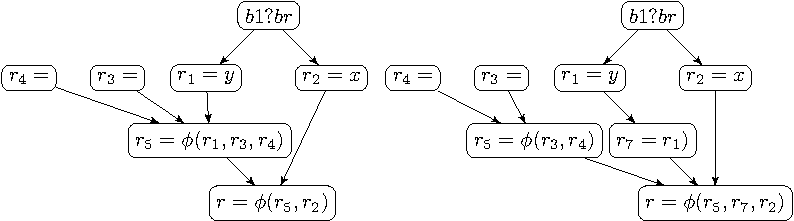
\includegraphics[scale=0.2]{phi_augmentation.pdf}
\caption{phi augmentation}
\label{fig:phi_aug}
\end{minipage}
\label{fig: phi_operations}
\end{figure}

\subsection{Scope}

The primary region candidate for if-converting is the extended hammock shape. This kind of region includes the traditional diamond (if-then-else). The hammocks are said to be extended because they can include an arbitrary number of basic blocks and back-edges are allowed, allowing a loop containing a set of branches to be converted into a single basic block without backedge coalescing.

The basic control structures that our analysis recognizes when is the Single Exit region formed from the minimal set of blocks between a branch point and a merge point.  Those are minimal single entry single exit regions because at this point nested regions were already if-converted. We define it as the region between a conditional block and the first common immediate postdominator of the taken path block and the fall-thru block.
Note that each path can contain zero or more basic blocks with incoming edges. Figure \ref{fig:hammocks} shows example of control flow regions considered for inclusion in the if-converted region.
As an optimization we allow two successive conditional blocks sharing one immediate post-dominator to be merged with logical operations after a normalization transformation. The normalization transformation ensures that conditional blocks sharing a same target can be merged by defining a wired $or$, or a wired $and$ share the same branch characteristics using branch reordering, test inversion or $de-morgan$ transformations.

The join basic block in the region is not part of the if-converted region, it is only used later in the if-conversion process for the SSA $\phi$ transformations. In structural analysis vocabulary, the abstract node is formed by the if-converted region without the join node.
Because, the join node is excluded from the if-converted region, while still part of the SSA process and iterated nested region formation, outer cyclic edges are allowed without the need for backeddge coalescing. 

    \subsection{SSA maintenance}

Consider a conditional branch depending on a predicate $p$ and a region starting at $BBhead$. Let $BBp$ be the set of single exit basic blocks $(BBi,\dots,BB_n)$ that are on the taken path if $p$ is true and $BBq$ be the set of single exit basic blocks $(BBj,\dots,BB_m)$ that are executed if $p$ is false. The merge point of the if-converted region is at $BBjoin$. We distinct 4 types of basic SSA transformation that the framework uses and produces:
\subsubsection{$\phi$ removal} (figure \ref{fig:phi_rem})
The join node of the considered region has two predecessors and $\phi$ instructions are of the form $r=\phi(r_1,r_2)$. After speculation of the definitions of $r_1$ and $r_2$ the instruction can be rewritten as $r=\psi(p?r_1,\overline{p}?r_2)$.
\begin{proof} Once $BBp$ and $BBq$ have been promoted into $BBhead$, $BBjoin$ has for only predecessor $BBhead$ so it is not in its dominance frontier. The $\phi$ is not necessary and is removed.
\end{proof}
\subsubsection{$\phi$ reduction} (figure \ref{fig:phi_red})
 The join node of the considered region has $n$ predecessors that have $\phi$ instructions of the form $r=\phi(r_1,r_i,r_j,\dots,r_n)$. After merging, the $\phi$s are rewritten $t=\psi(p?r_i,overline{p}?r_j)$ and a new $\phi$ $r=\phi(r_1,t,\dots,r_{n-1})$ is created with one operand less. The $\psi$ instruction is inserted after the speculated $r_i$ and $r_j$ definitions into $BBhead$.
\begin{proof} $BBjoin$ is still in the dominance frontier of $BBhead$, A $\phi$ must be redefined with the new definitions. The two corresponding $\phi$ edges from $BBq$ and $BBp$ can be replaced by the $BBhead$ edge.
The join block $E$ has $n$ predecessors with $n$ > 2, and $n$ blocks in its dominance frontier if it contains $\phi$s.
\end{proof}
\subsubsection{$\phi$ augmentation} (figure \ref{fig:phi_aug})
The objective is to remove incoming edges into the region. 
Consider a join node with $n$ predecessors among which $p$ is duplicated into $q$.  The join node of the considered region have $\phi$ instructions of the form $r=\phi(r_1,p,r_i,r_j,\dots,r_{n-1})$. The instruction is rewritten $t=select(p,r_i,r_j)$ and \mbox{$r=\phi(r_1,t,q,\dots,r_n)$}. 
\begin{proof}The duplicated blocks are new dominators of $BBjoin$ that define new $defs$. These blocks are now in the dominance frontier of $BBjoin$. SSA is maintained with new $\phi$ upgraded with the new reaching points.
Since the algorithm works the control flow in post order mode, the dominator tree doesn't change, and it's possible to maintain the SSA locally to the inner region. By recurence the if-converted region can be in turn be optimized out if it's head belongs to the dominance frontier of an outer region.
\end{proof}
Note that block duplication doesn't necessary implies more code size, since data flow dependencies are broken, noew oportunities for propagation or scalar optimisation arise. Here the local $t$ appears temporary, since $r2$ can be propagated into the $\phi$.

\section{SSA promotion}

To know the values that need to be conditionally written, we only need to look at the defining instructions of the $\phi$ instructions. By elimination, all temporaries that do not have a join point into the considered region are unconditionally speculated during the SSA transformations processes.

If-conversion converts control dependencies into data dependencies by computing a condition for the execution of each operation \cite{Schlansker-predicated}. Using our SSA framework, only operands from $\phi$ operations are considered to be conditional. This is an important advantage over traditional if-conversion algorithms that marks all instructions in a conditional basic block as dependent on the predicate. When considering dependency on a predicate we just walk from the $\phi$ uses to their definition points. All instructions are unconditionally speculated, but only those that are used in $\phi$ merge points that SSA exposes the conditional merging of values and generation of conditional moves.

Our algorithm is applied iteratively on a control flow in SSA form until no more reductions are possible. The quality of the SSA taken as input does not affect the correctness of the algorithm: if the control flow is in pruned SSA, i.e two paths $x->+z$ and $y->+z$ converge at node z, then a $\phi$ node is inserted at z only if z is alive in or after z. if which case x and y are promoted and no $select$ operation is generated. if the SSA is minimal, a $select$ instruction would be generated and removed by dead code. Inserting dead code from minimal SSA only introduces noise in the local scheduling heuristics because of the false data dependencies.

The basic idea behind the SSA transformations is to replace $\phi$ operations by predicated instructions merging into a $\psi$ or speculated instructions merging into a $select$ equivalent instructions, while maintaining the SSA properties. In figure \ref{fig:ssa} the conditional assignment uses a new temporary $r4$. Since the basic block containing the $\phi$ now has two incoming edges, a new $\phi$ is created to replace the former within the newly locally maintained SSA region.

The $select$ generation being done after instruction selection, the if-conversion framework can take opportunities for local optimizations such as conditional constant propagation like the $r2=2$ assignment in figure \ref{fig:ssa} if it can be absorbed by the $select$ instruction. Doing such optimizations locally enables the heuristics to be more precise in the formation of candidate if converted new regions.

\subsubsection{Partial redefinition}

$\psi$ operation exposes new control flow dependencies to the data flow, by expressing the merge of two definitions. Note that the order of the partial definition is important, so a definition partially redefines the preceding ones. We use this propriety to speculate the first definitions, so it becomes speculated instead of disjoint. This local optimisation allow to remove a predicate dependency but also creates a new partial dependency (predicates are not disjoint). Removing a predicate dependency is usually best because it allows to schedule the predicate computation earlier.

\begin{figure}
\footnotesize
\begin{minipage}{6cm}
$ p \cond x_1 = a + b $ \\
$ \overline{p} \cond x_2 = c $ \\
$ x = \psi(p \cond x_1, \overline{p} \cond x_2) $ \\
\caption{disjoint predicates}
\end{minipage}
\begin{minipage}{6cm}
$ x_1 = a + b $ \\
$ \overline{p} \cond x_2 = c $ \\
$ x = \psi(T \cond x_1, \overline{p} \cond x_2) $ \\
\caption{optimized order predicates}
\end{minipage}
\end{figure}

$T$ represents the $True$ predicate. This optimization is usefull to save one predicate register and to reduce the dependence height between a predicate definition in its use. 
The $\psi$ definition is defined on the $T$ predicate set, therefore it is speculable, as shown here:

     \subsubsection{$\psi$ speculation properties}

Since the algorithm process the regions from inner to outer, conditional operations will be in turn speculated or reconditionalized with a new condition. We define here $\psi$ operand promotion rules.

Consider the code \ref{fig:nested_psi}  containing a subregion already processed

Note the value produced in (4) is not defined for $p \& \overline{c}$ and $overline{p} \& \overline{c}$. Gladly all operations in defines $d_2 the \overline{c}$.

\subsubsection{$\psi$ predication properties}

If the instructions are not speculable, then they must be predicated:
The c condition must be merged with all conditions under which the phi operands are used. here d1 uses !p, so the psi can be rewritten as

We can see with this example that the decision to speculate or predicate can be done at the level of each joining definition, allowing a mix of them in the final program. The advantage to speculation over predication is a reduced dependency length. The disadvantage of speculation is that it increases register pressure untill the merge point, and put long latencies operation on the critical path.
 
\begin{figure}
\footnotesize
\begin{minipage}[b]{4cm}
$ if (c) $ \\
$ \{ $ \\
\hspace*{2mm}$ x_1 = a + b $ \\
\hspace*{2mm}$ \overline{p} \cond x_2 = c $ \\
\hspace*{2mm}$ x = \psi(T \cond x_1, \overline{p} \cond x_2) $ \\
\hspace*{2mm}$ d_1 = use (x) $ \\
$ \} $ \\
$ else $ \\
\hspace*{2mm}$ d_2 = 3 $ \\
$ d = \phi(d_1,d_2) $ \\
\caption{nested if}
\label{fig:nested_psi}
\end{minipage}
\begin{minipage}[b]{4cm}
$ x_1 = a + b $ \\
$ \overline{p} \cond x_2 = c $ \\
$ x = \psi(T \cond x_1, \overline{p} \cond x_2) $ \\
$ d_1 = use (x) $ \\
$ \overline{c} \cond d_2 = 3 $ \\
$ d = \psi(T \cond d_1, \overline{c} \cond d_2) $ \\
\caption{speculated nested if}
\label{fig:nested_psi_speculated}
\end{minipage}
\begin{minipage}[b]{4cm}
$ p_1 = \overline{p} \& {c} $ \\
$ c \cond x_1 = a + b $ \\
$ p_1 \cond x_2 = c $ \\
$ x = \psi(c \cond x_1, p_1 \cond x_2) $ \\
$ d_1 = use (x) $ \\
$ \overline{c} \cond d_2 = 3 $ \\
$ d = \psi(T \cond d_1, \overline{c} \cond d_2) $ \\
\caption{predicated nested if}
\label{fig:nested_psi_predicated}
\end{minipage}
\end{figure}

\subsubsection{Predicate merging}

During the regions formation, subregions containing a block that is reached from two conditions can be optimized by merging predicates. A new predicate is computed using a logical operation on both basic blocks' predicates after a normalization pass. Simple logical operations are usually caught as a peephole or during the instruction selection mechanism, but making it part of the if-conversion process allows it to handle more complex regions because our predicate merging algorithm is not limited to basic blocks that only define predicates, making instructions depending of predicates merge part of the generic SSA speculation framework. However, this transformation is very sensitive to biased branches since each conditional operation now depends on two predicates instead of one that cannot be scheduled together because of the computation of the logical operation making it more difficult to compensate for the branch removal. In order to avoid artificially increased dependence height we exclude from this promotion predicates that depend on long latency operations.
Because of new data dependencies introduced by the new computed predicate the performance contribution of this transformation mainly comes from the branch removal (two conditional branches and two direct branches are removed from a if-converted region whose predicates have been merged) rather than local ILP. Predicate promotion and merge is more effective in loop nest regions where more optimizations may extract ILP from it, for example modulo scheduling can extract ILP from such if-converted body by overlapping different iterations. 

\subsubsection{Block duplication}

Block duplication is used to remove side edges and to remove the constraints on control dependencies that enable the algorithm to find a set of basic blocks to if-convert. Unless applied carefully, we were afraid that block duplication could be the cause of code bloating without a performance counterpart. However experience has shown that when applied carefully it can be the source of very efficient if-conversion. Consider for example in the figure \ref{fig:bbdup}. Since we are if-converting from the inner most regions, the algorithm first considers the region {BB3,BB4,BB5,BB6,BB7}, and discards the edge coming from BB2 by duplicating BB6 into BB8. The $\phi$ becomes a move in the duplicated block with a renamed definition. The new $\phi$ operands are updated from the new edge. Note that in the implementation the block does not need to be created since it will be next promoted into BB3. We have two nested hammocks and the process can restart. The dependency that we removed in the control flow is now expressed as a data dependency between the two $select$ instructions.

The algorithm to perform SSA block duplication is decomposed into three steps: 
\begin{itemize}
\item Extract the $\phi$s 's def to be conditionalized from the duplicated block creating a $move$ instruction and a new reduced $\phi$ (or two $move$ instructions if the duplicated block had only two incoming edges).
\item Then the $\phi$s in the tail basic block are augmented with the new def created by the new repair instruction. If the $\phi$ was live-out after the tail block a move must be inserted to avoid propagating renaming outside of the region considered. 
\item The last step consists of renaming the new definitions to keep the region into SSA.
\end{itemize}

\begin{figure}[th]
\begin{minipage}[b]{3cm}
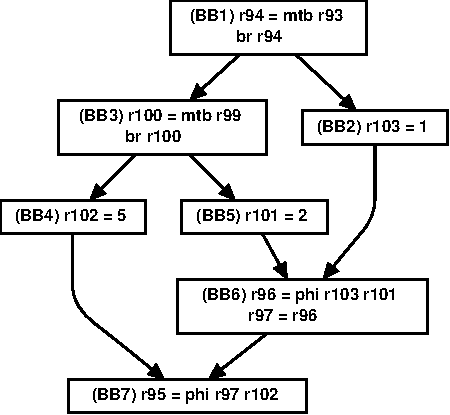
\includegraphics[scale=0.3]{g1.pdf}
\end{minipage}
\begin{minipage}[b]{3cm}
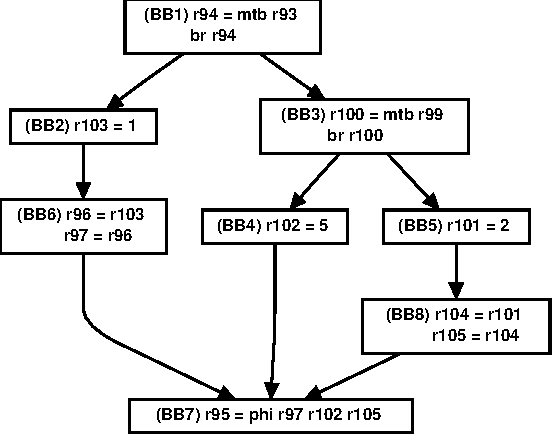
\includegraphics[scale=0.3]{g2.pdf}
\end{minipage}
\begin{minipage}[b]{3cm}
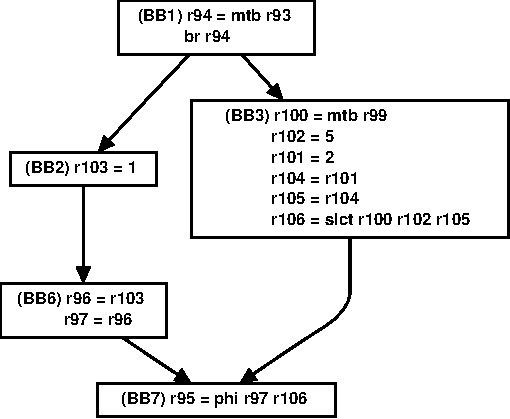
\includegraphics[scale=0.3]{g3.pdf}
\end{minipage}
\begin{minipage}[b]{3cm}
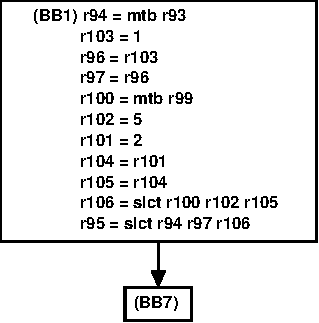
\includegraphics[scale=0.3]{g4.pdf}
\end{minipage}
\caption{Side entry removal using block duplication}
\label{fig:bbdup}
\end{figure}

\section{Hyperblock Region contruction}

These operation are performed iterativelly on post order, consequently one of the propriety of the algorithms is that psi can be predicated. A Partial out of SSA can be iteratively performed on those regions by removing the $\phi$s and maintening a correct SSA internal representation. The algorithm takes SSA as input and produces SSA if a select instruction is available or $\psi$-SSA if predicated instructions are available. 

\subsubsection{Running example}
Consider the control flow transformations for the $wc$ program (figure \ref{fig:wc_cfg}).
(The formation of conditional instructions will be detailed in the next section).
 The postorder list of the basic nested regions is {\em BB11, BB17, BB16, BB14, BB10, BB9, BB6, BB2} (The start of the nested regions are represented by the circle nodes). First, for BB11, BB12 is promoted and BB2 becomes a fall-thru of BB11 . For the region starting at BB17, BB19 cannot be promoted because of the side entry coming from BB15. BB16 is the start of a logical region from the two predicates BB16 BB17. A new predicate is computed from the one defined in BB17 and the one defined in BB16. BB17 is promoted and the registers alive in BB19 are conditionalized with the new predicate. The process continues on BB16. BB19 is duplicated to remove the side edge. BB14 is the head of the newly created region where BB15, BB16 and BB17 can be promoted. From BB9 a logif predicate is computed with the one in BB10. Instructions in BB14 are conditionalized on this new predicate and BB10 promoted, forming a new hammock at BB9 with BB14 and BB11 that can be promoted. The last candidate, BB2 is the start of a region that cannot be promoted, because of the call into BB3. the region is if-converted, leaving a single back-edge, removing 7 branches inside the body loop.

This is a good if-conversion example because the original control flow is complex enough to stress the algorithm. In a loop region, if-conversion is critical to extract required performance. It is also a good balance between
 memory operations and register operations. (Another reason is that this example is very popular in the if-conversion literature). 
After our transformations, the static $wc$ loop schedule is 23 cycles instead of 31 cycles. The last basic blocks $BB2,3,4,5$ could not be if-converted because of the presence of a call instruction.

\begin{figure}[h]
\begin{center}
\( \begin {tabular}{cc}
\\
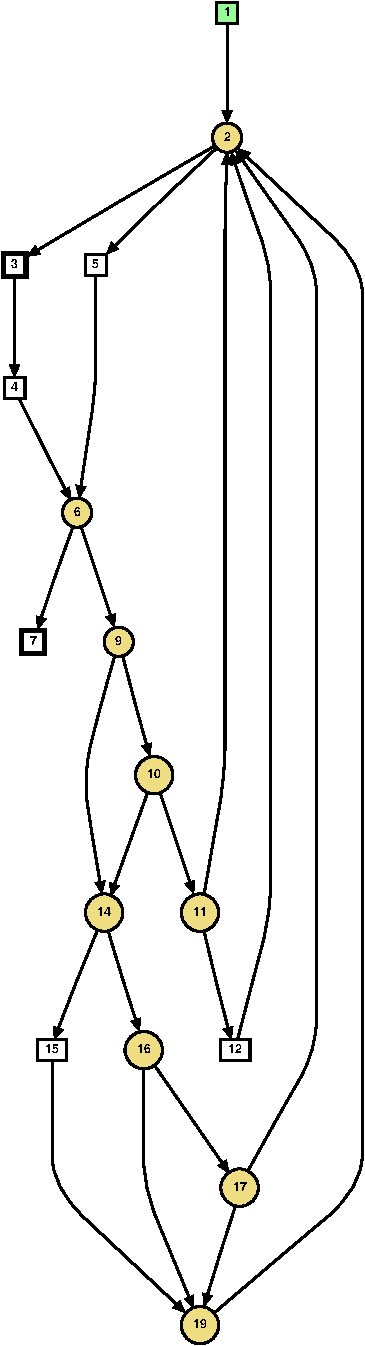
\includegraphics[scale=0.6]{graph1.pdf} &
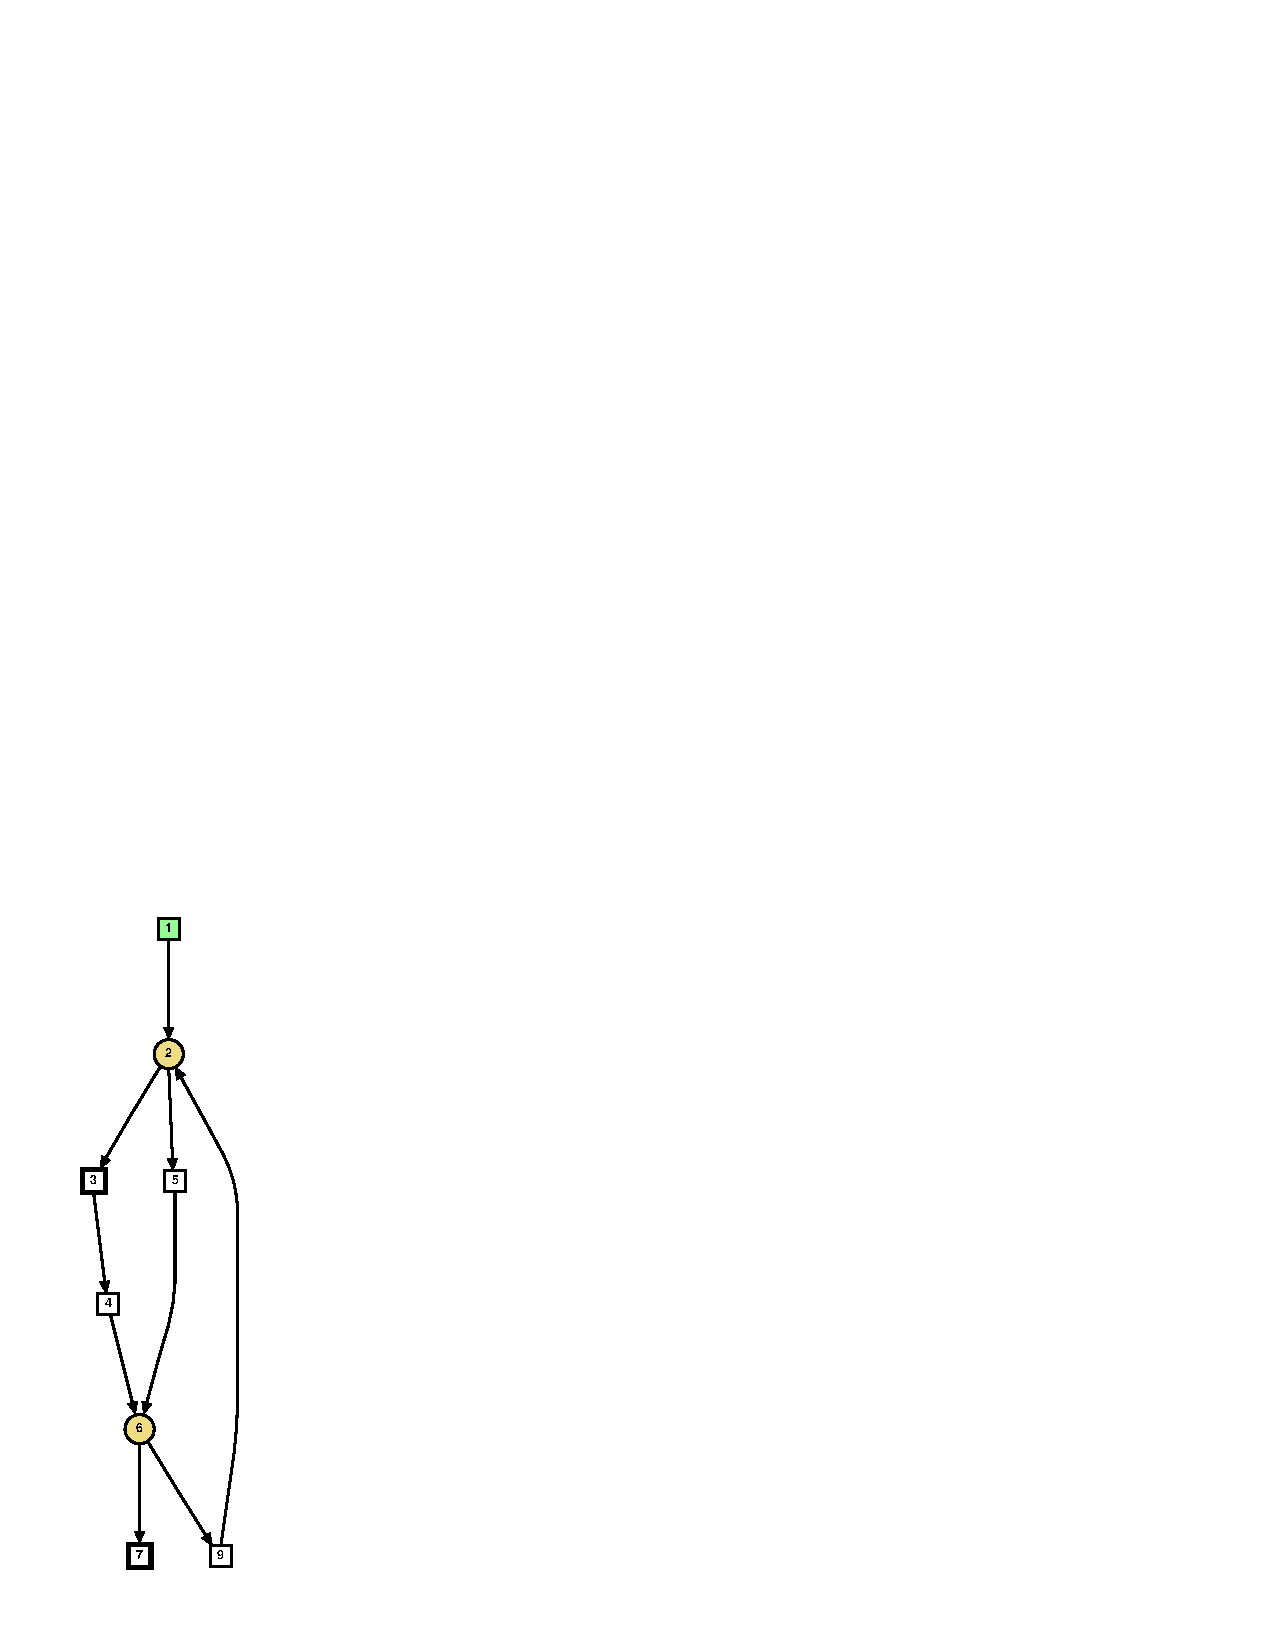
\includegraphics[scale=0.6]{graph7.pdf}
\\
\mbox{\bf before if-conversion} & \mbox{\bf after if-conversion}
\\
\mbox{31 cycles} & \mbox{23 cycles} 
\end{tabular} \)
\end{center}
\caption{wc.c control flow}
\label{fig:wc_cfg}
\end{figure}



